

\chapter{Spear Benchmarks} 
\label{app:spear_alltoallv_benchmarks}

The data in this appendix was acquired on the FSU Spear cluster. It is provided for comparison with \cite{BolligFlyerErlebacher2012}.

\section{Spear Scaling with MPI\_Alltoallv}

Although the Spear cluster is not identical to Keeneland, it runs similar GPU hardware allowing for direct comparison

\begin{figure}
\centering
\begin{subfigure}[t]{0.425\textwidth}
\centering
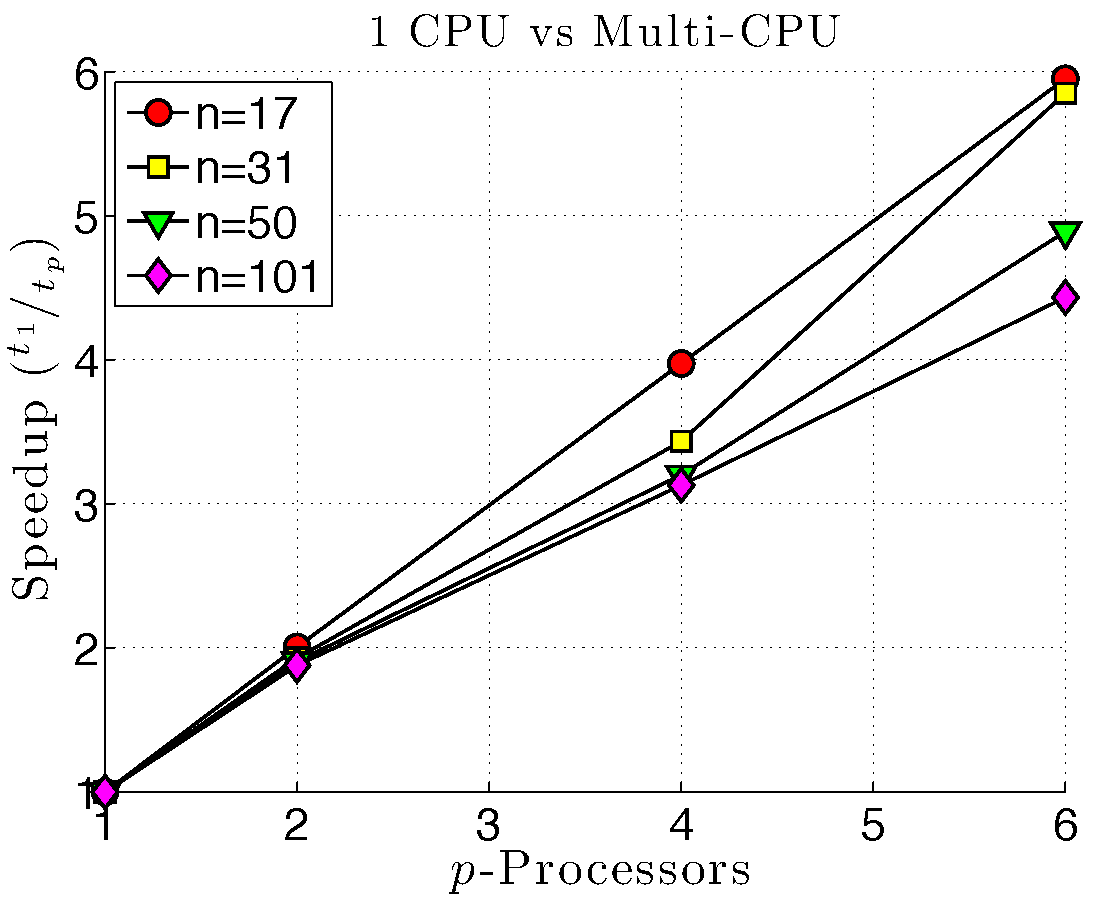
\includegraphics[width=1.0\textwidth]{../figures/spear_results/alltoallv_vortex/speedup_1CPU_vs_NCPU.pdf}
\caption{Multi-CPU strong scaling on Spear for one warp per stencil}
\label{fig:spear_alltoall_multicpu_scaling}
\end{subfigure} 
\begin{subfigure}[t]{0.425\textwidth}
\centering
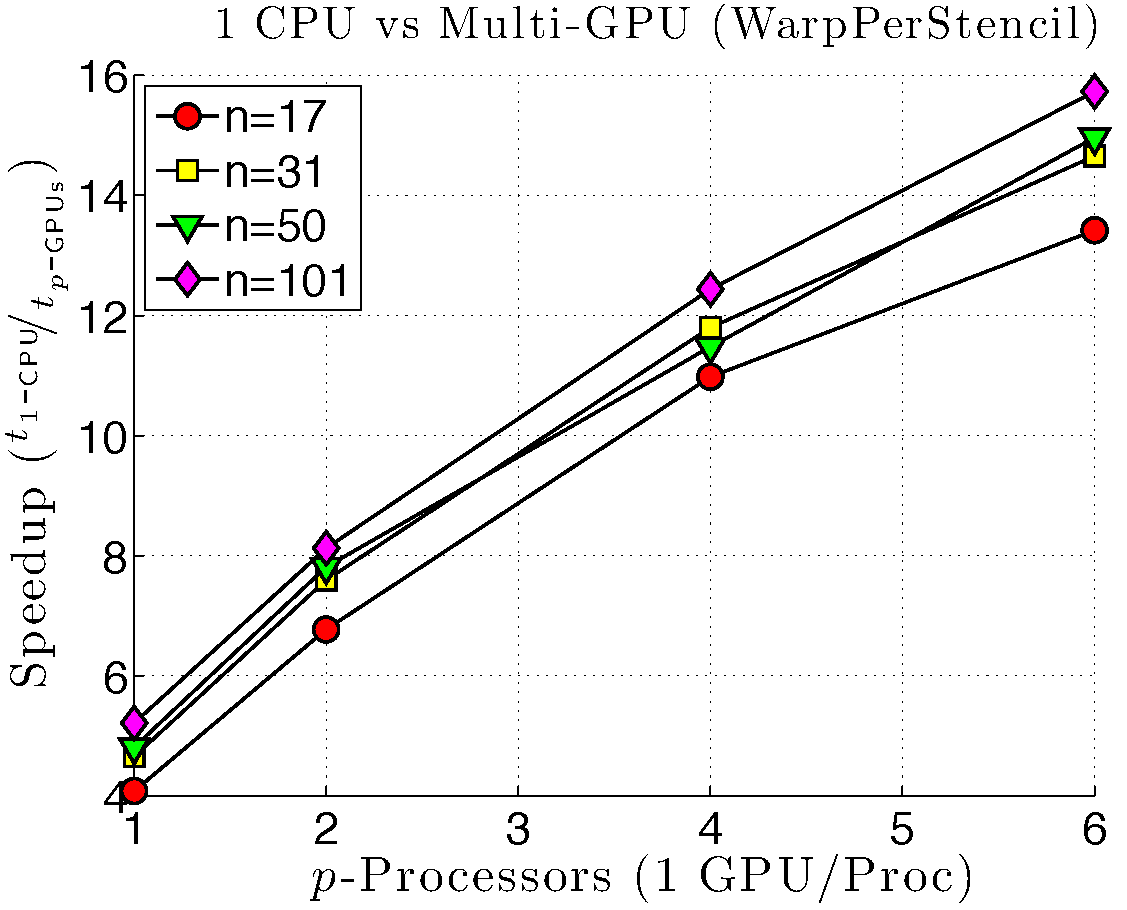
\includegraphics[width=1.0\textwidth]{../figures/spear_results/alltoallv_vortex/speedup_1CPU_vs_NGPU_WarpPerStencil.pdf}
\caption{Multi-GPU strong scaling vs one CPU on Spear for one warp per stencil}
\label{fig:spear_alltoall_multigpu_vs_cpu_scaling}
\end{subfigure} 
\begin{subfigure}[t]{0.425\textwidth}
\centering
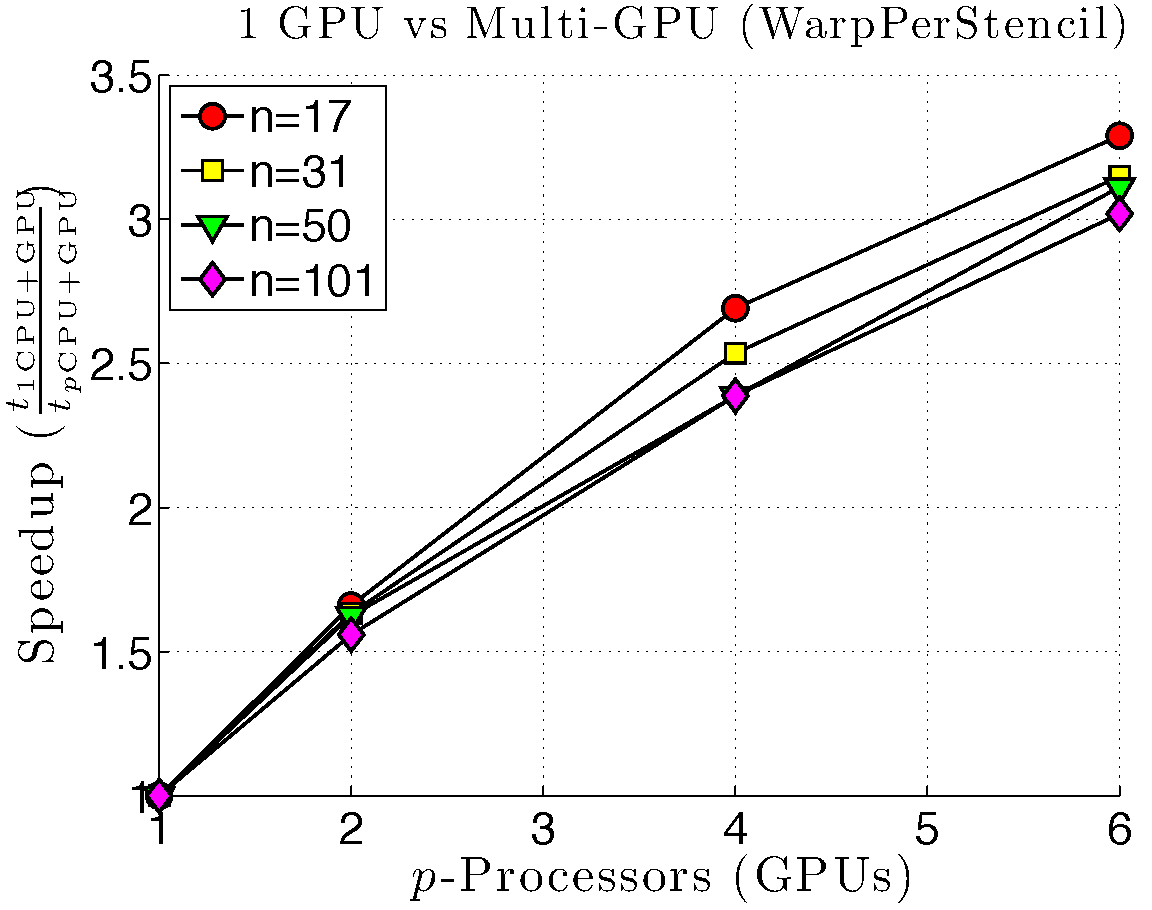
\includegraphics[width=1.0\textwidth]{../figures/spear_results/alltoallv_vortex/speedup_1GPU_vs_NGPU_WarpPerStencil.pdf}
\caption{Multi-GPU strong scaling vs one GPU on Spear for one warp per stencil}
\label{fig:spear_alltoall_multigpu_vs_gpu_scaling}
\end{subfigure} 
\caption{Distributed CPU and GPU scaling on the FSU Spear cluster.}
\end{figure} 



\begin{figure}
\centering
\begin{subfigure}[t]{0.425\textwidth}
\centering
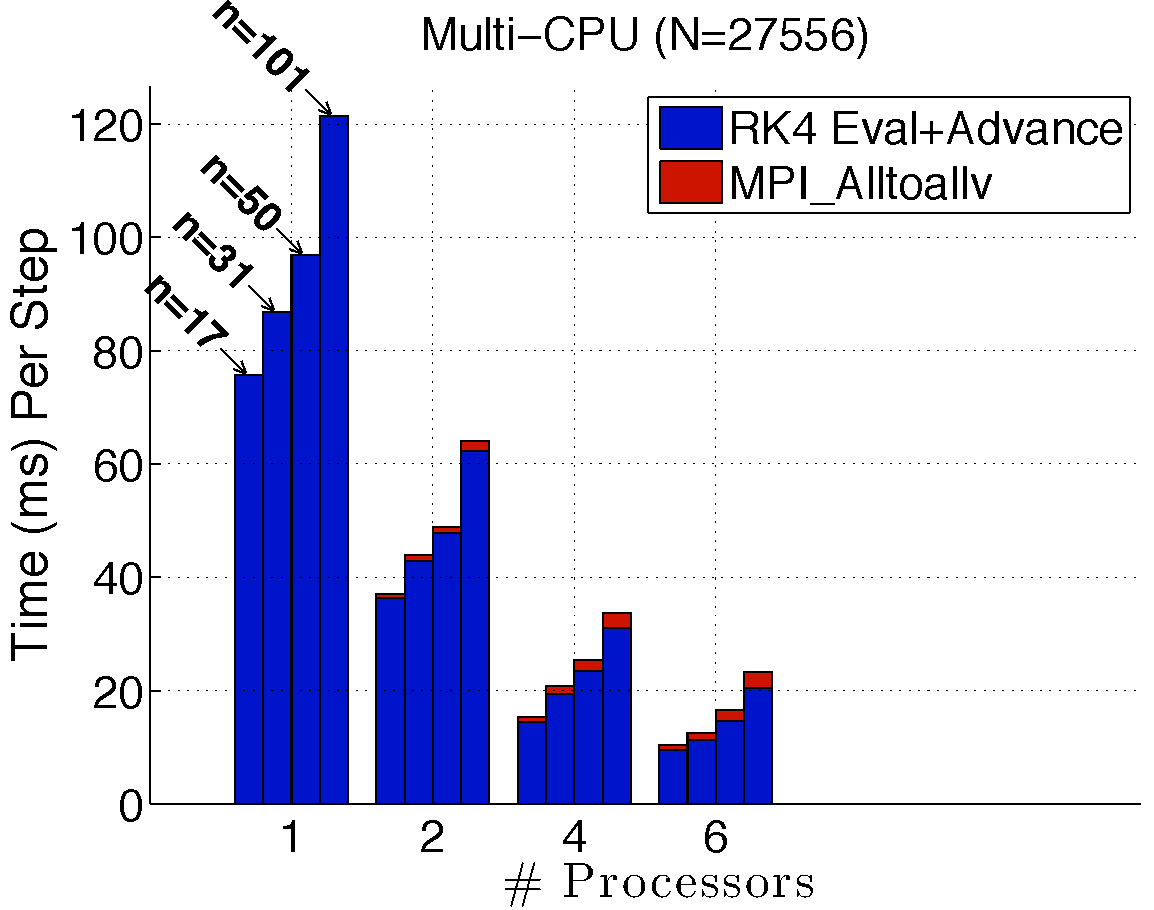
\includegraphics[width=1.0\textwidth]{../figures/spear_results/alltoallv_vortex/multiCPU_costs.pdf}
\caption{Multi-GPU strong scaling vs one GPU on Spear for one warp per stencil}
\label{fig:spear_alltoall_multigpu_vs_gpu_scaling}
\end{subfigure} 
\begin{subfigure}[t]{0.425\textwidth}
\centering
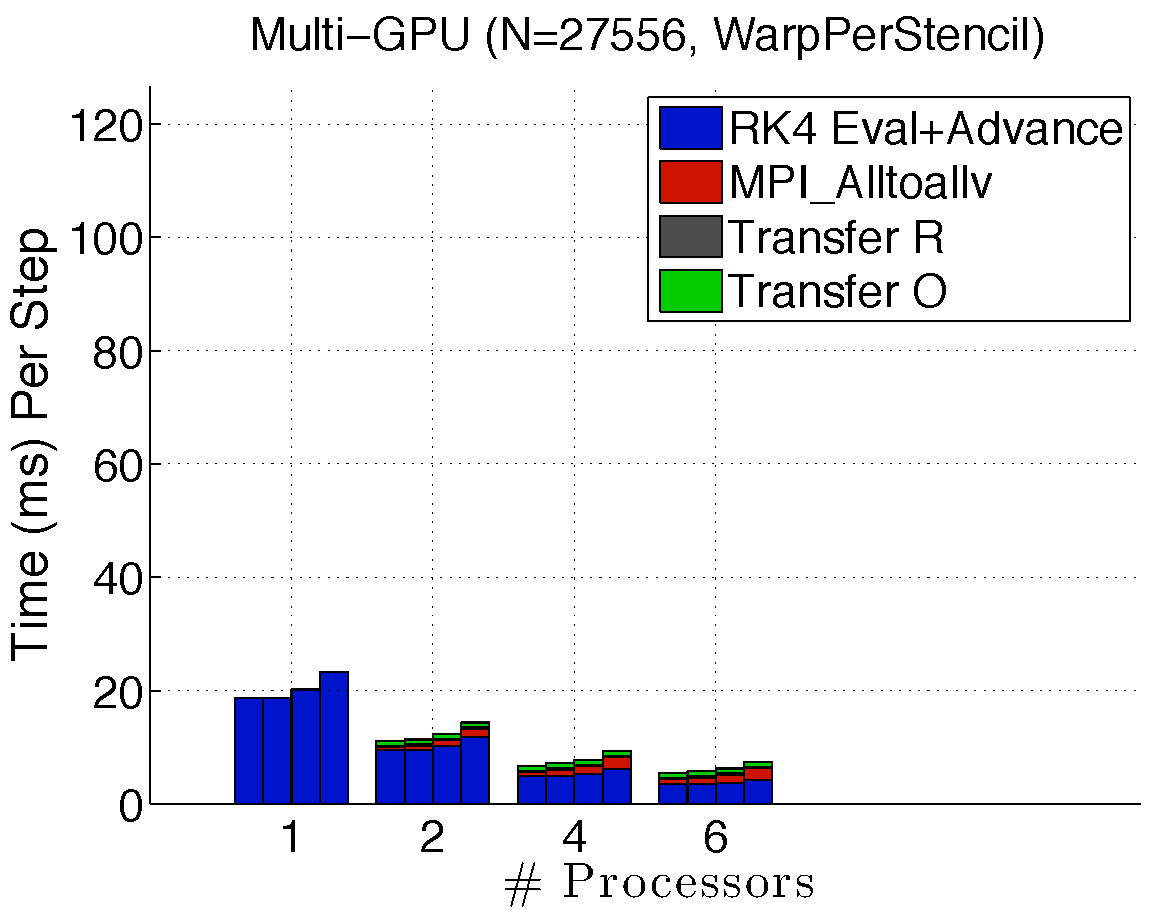
\includegraphics[width=1.0\textwidth]{../figures/spear_results/alltoallv_vortex/multiGPU_warp_costs.pdf}
\caption{Multi-GPU strong scaling vs one GPU on Spear for one warp per stencil}
\label{fig:spear_alltoall_multigpu_vs_gpu_scaling}
\end{subfigure} 
\begin{subfigure}[t]{0.425\textwidth}
\centering
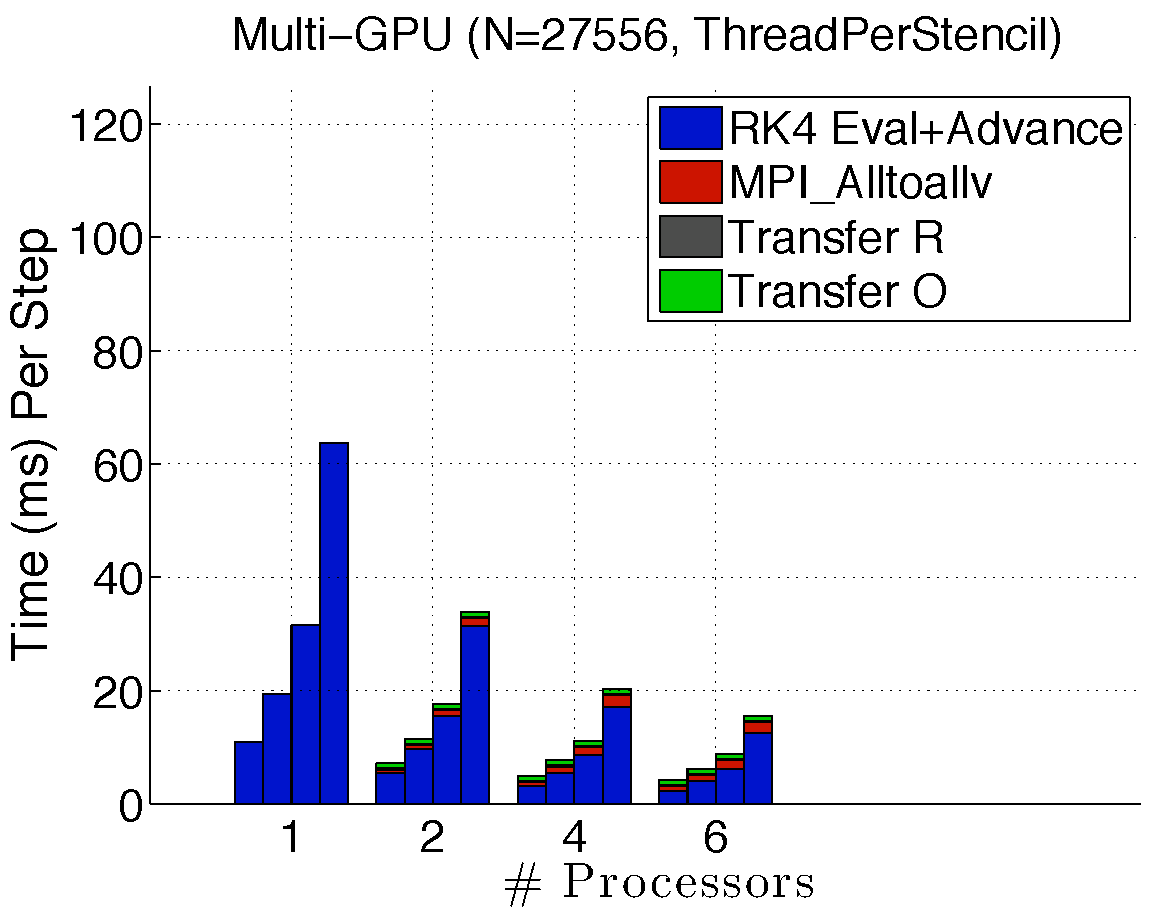
\includegraphics[width=1.0\textwidth]{../figures/spear_results/alltoallv_vortex/multiGPU_thread_costs.pdf}
\caption{Multi-GPU strong scaling vs one GPU on Spear for one thread per stencil}
\label{fig:alltoall_multigpu_vs_gpu_scaling}
\end{subfigure} 
\end{figure} 


\section{Single GPU SpMV on Spear}

These results were run on Spear. MPI communication is done with an MPI\_alltoallv collective. The test case is the vortex roll-up. 

Figure~\ref{fig:spear_alltoall_1proc_warp} 

\begin{figure}
\centering
\begin{subfigure}[t]{0.425\textwidth}
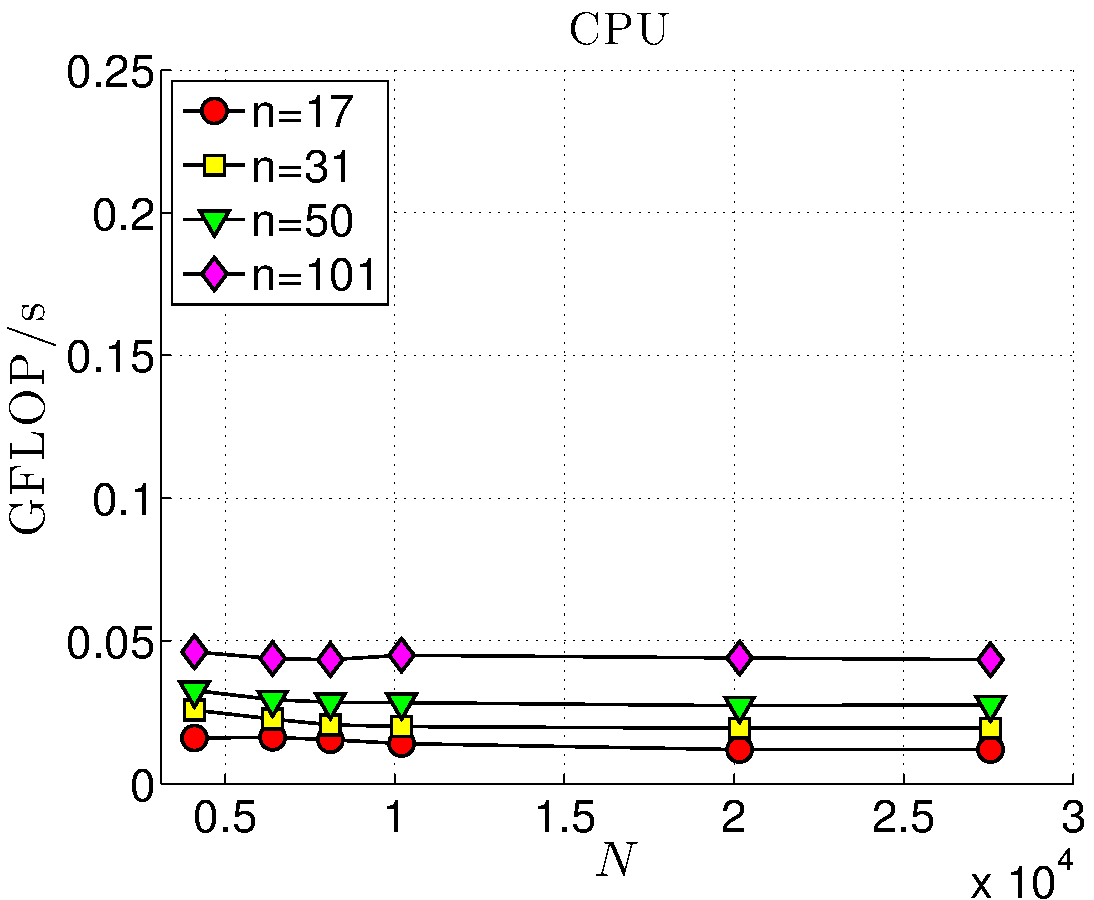
\includegraphics[width=1.0\textwidth]{../figures/spear_results/vortex/gflops_cpu_1proc_oneWarpPerStencil-eps-converted-to.pdf}
\caption{One warp per stencil kernel on one GPU in Spear \authnote{TODO: update} }
\label{fig:spear_alltoall_1proc_warp}
\end{subfigure} 

\begin{subfigure}[t]{0.425\textwidth}
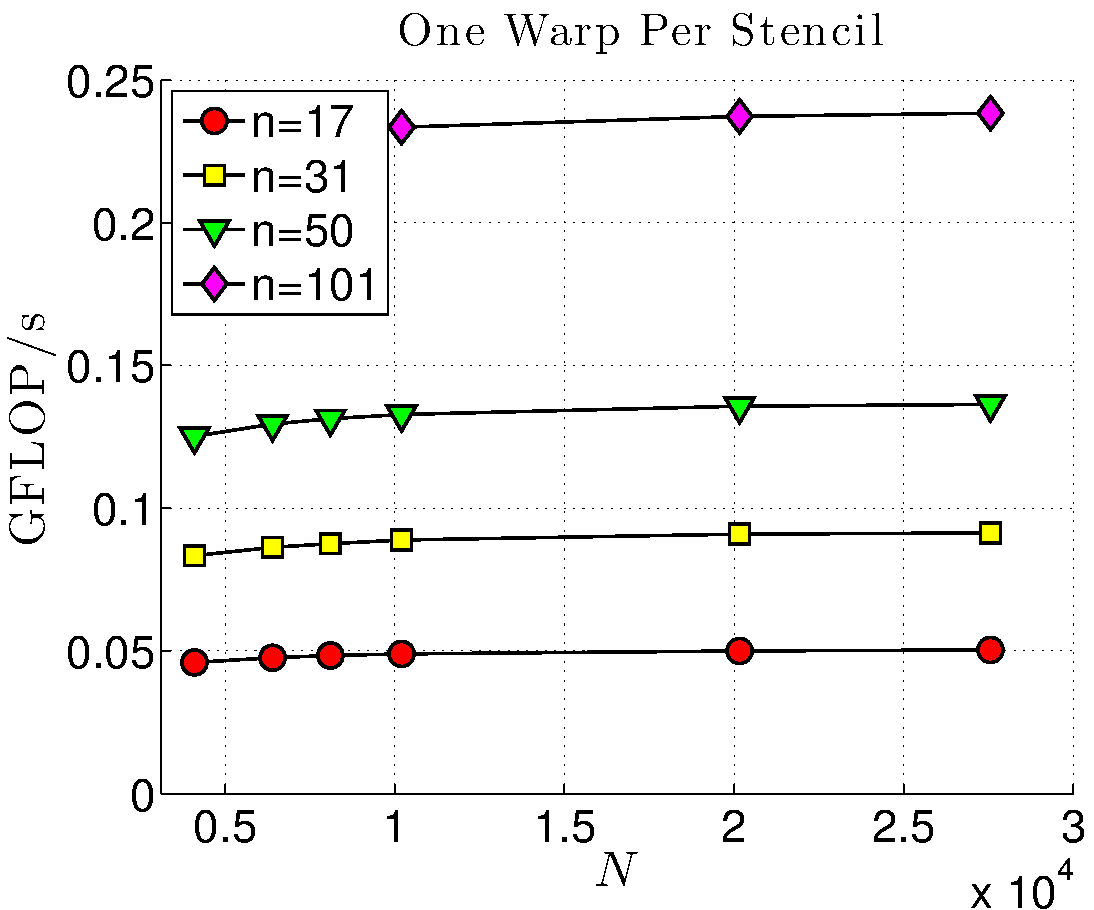
\includegraphics[width=1.0\textwidth]{../figures/spear_results/vortex/gflops_gpu_1proc_oneWarpPerStencil-eps-converted-to.pdf}
\caption{One warp per stencil kernel on one GPU in Spear}
\label{fig:spear_alltoall_1proc_warp}
\end{subfigure} 
\begin{subfigure}[t]{0.425\textwidth}
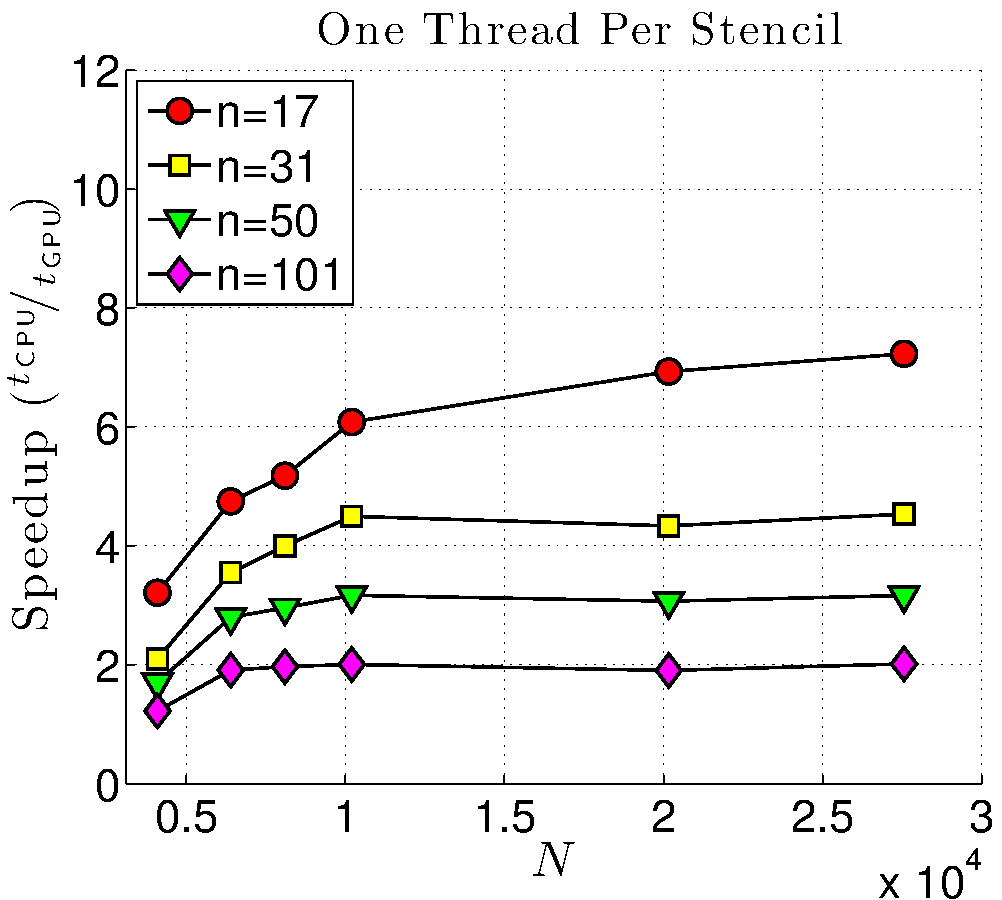
\includegraphics[width=1.0\textwidth]{../figures/spear_results/vortex/speedup_1proc_oneThreadPerStencil-eps-converted-to.pdf}
\caption{One warp per stencil kernel on one GPU in Spear}
\label{fig:spear_alltoall_1proc_warp}
\end{subfigure} 
\end{figure} 

\begin{figure}
\centering
\begin{subfigure}[t]{0.425\textwidth}
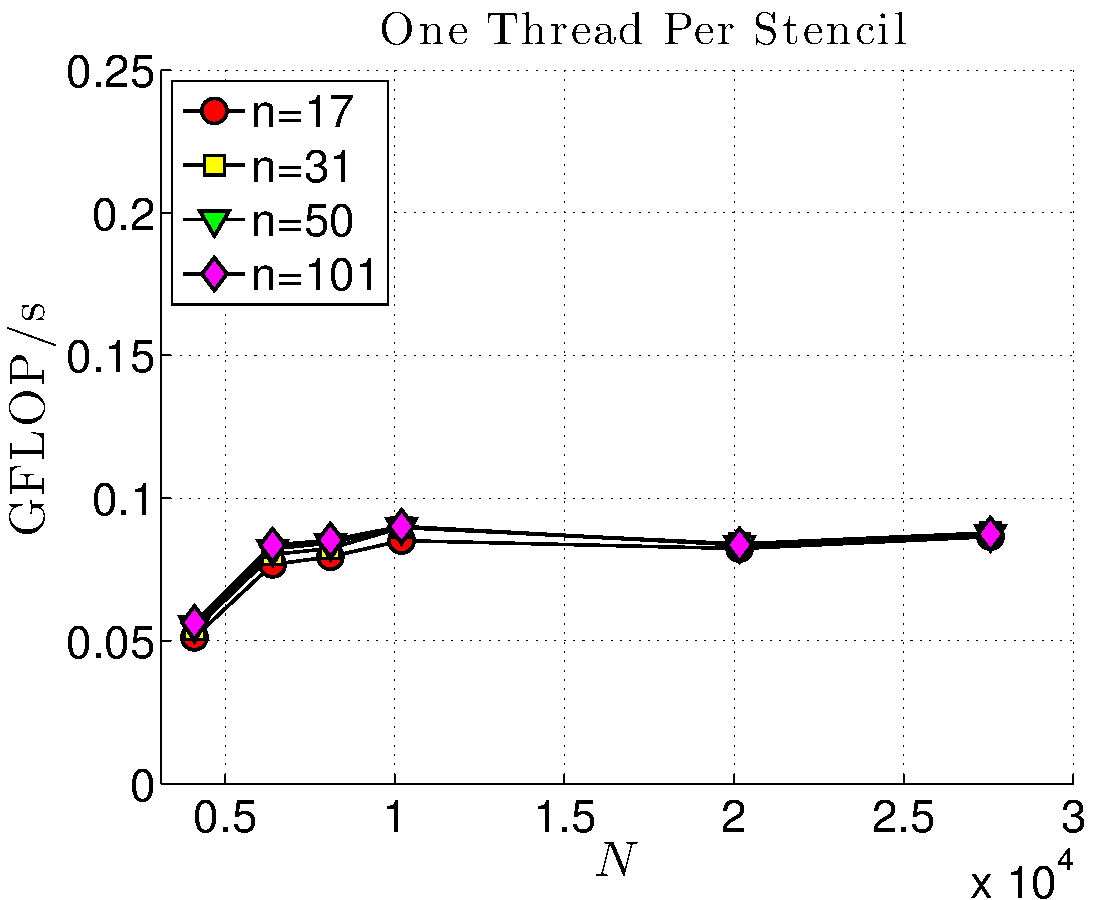
\includegraphics[width=1.0\textwidth]{../figures/spear_results/vortex/gflops_gpu_1proc_oneThreadPerStencil-eps-converted-to.pdf}
\caption{One warp per stencil kernel on one GPU in Spear}
\label{fig:spaer_alltoall_1proc_warp}
\end{subfigure} 
\begin{subfigure}[t]{0.425\textwidth}
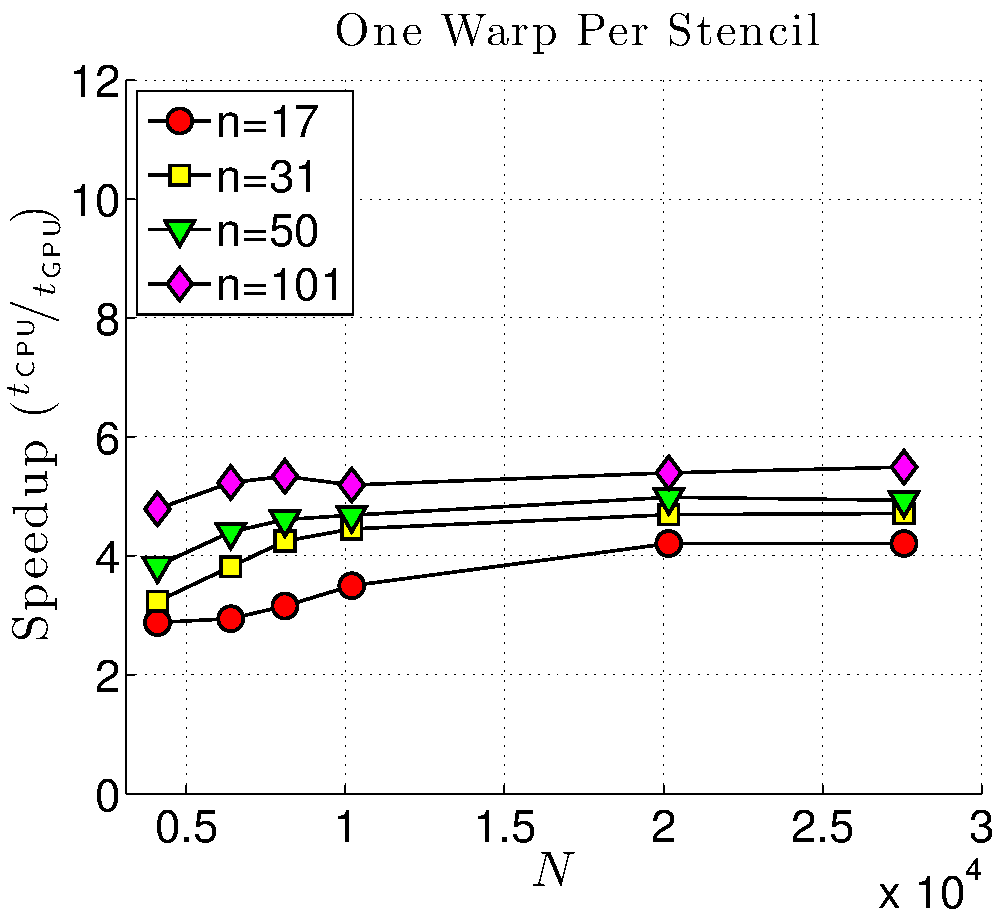
\includegraphics[width=1.0\textwidth]{../figures/spear_results/vortex/speedup_1proc_oneWarpPerStencil-eps-converted-to.pdf}
\caption{One warp per stencil kernel on one GPU in Spear}
\label{fig:spear_alltoall_1proc_warp}
\end{subfigure} 
\end{figure}

\section{ViennaCL}

These benchmarks compare performance of a single SpMV executed on Spear. Each data point is the average over 10 executions. The GPU is primed by an iteration before benchmarking begins. 

\begin{figure}
\centering
\begin{subfigure}[t]{0.48\textwidth}
\centering
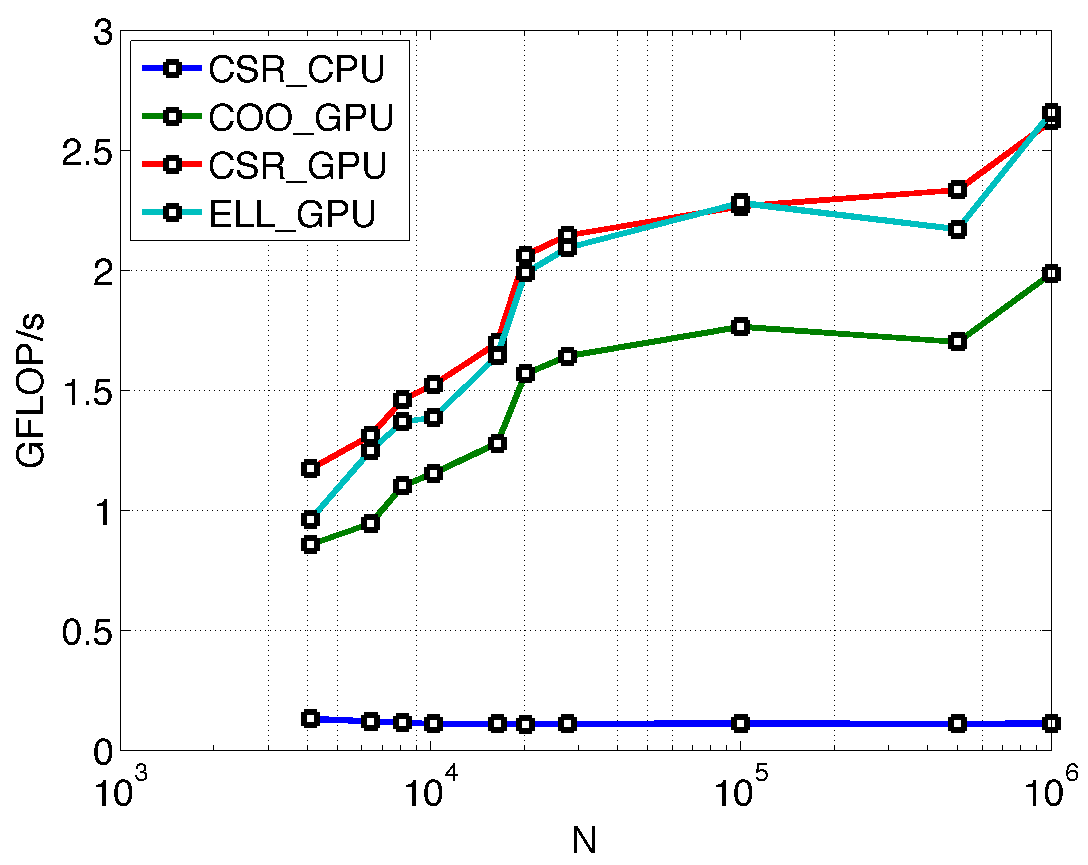
\includegraphics[width=1.0\textwidth]{../figures/spear_results/spmv/spmv_vcl_gflops-eps-converted-to.pdf}
\caption{SpMV Performance of the ViennaCL CSR, COO and ELL formats versus the BOOST::uBLAS CSR format.}
\label{fig:spear_vcl_gflops}
\end{subfigure} 
\begin{subfigure}[t]{0.48\textwidth}
\centering
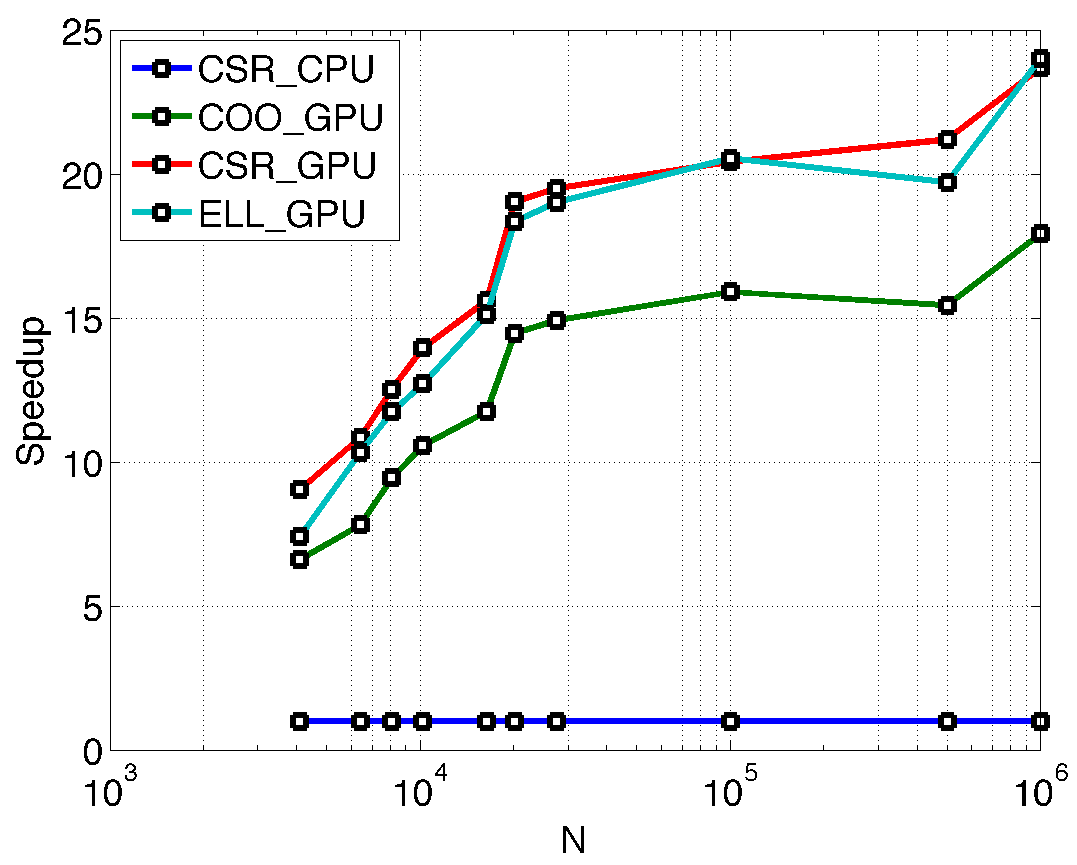
\includegraphics[width=1.0\textwidth]{../figures/spear_results/spmv/spmv_vcl_speedup-eps-converted-to.pdf}
\caption{Speedup relative to the BOOST::uBLAS CSR implementation on the CPU.}
\label{fig:spear_vcl_speedup}
\end{subfigure} 
\caption{Single GPU SpMV performance for ViennaCL vs BOOST::uBLAS on the Spear cluster (FSU) for $n=50$. }
\end{figure}


